%gibt an: Papierformat, einseitiger Druck, Schriftgr��e
\documentclass[a4paper,oneside,titlepage,12pt]{article}
%-------------------------------------------------------------------
\usepackage[a4paper, top=2cm, footskip=0pt, headheight=0.8cm, headsep=0.6cm, lmargin=3cm, rmargin=2cm]{geometry}
\usepackage{graphicx}
\usepackage{helvet}
\usepackage{amsmath}
\usepackage{amsthm}
\usepackage{amssymb}
\usepackage{hyperref} 
\usepackage[right]{eurosym}
\usepackage[latin1]{inputenc}

%--------------------------------------------------------------------
\renewcommand{\baselinestretch}{1.2}

\begin{document}
%--------------------------------------------------------------------
%Titelseite
\begin{titlepage}
	
\includegraphics{grafiken/HTW-Logo.png}
	%
\includegraphics[width=.3\textwidth]{grafiken/HTW-Logo.png}
	\vspace*{3cm}
	\begin{center}
		\Huge{Benutzerdokumentation\\} \vspace*{1cm}
		\huge{Case-Gruppe 04\\}
		\vspace*{1cm}
		\Large{
			Modul: Software Engineering II\\}
		\vspace*{2cm}
		\normalsize{
			Studiengang Informatik\\
		}
	\end{center}
	\vspace{2cm}
\begin{center}
\large{Sommersemester 2014}
\end{center}
	\vspace*{3cm}



\end{titlepage}

\thispagestyle{empty}\clearpage

%-----------------------------------------------------------------------------------------------------------------------------------
%\rmfamily \pagestyle{fancy} \setcounter{secnumdepth}{4}
\newtheorem{satz}{Satz}
\newtheorem{lemma}[satz]{Lemma}
\newtheorem{folgerung}[satz]{Folgerung}
\theoremstyle{definition}
\newtheorem{definition}[satz]{Definition}
\numberwithin{equation}{section}
\renewcommand{\proofname}{Beweis}

\pagenumbering{roman}\setcounter{page}{3} \tableofcontents
\newcounter{roemisch} \setcounter{roemisch}{\value{page}}
\clearpage

\setcounter{page}{2} \pagenumbering{arabic}

\section{Einleitung}
Das entwickelte Software-System dient zur Verwaltung von Beleggruppendaten und
besteht aus genau 2 Programmen. Eines f�r die Studenten zum Anmelden und
Verwalten ihrer eigenen Gruppe und zum anderen ein Programm f�r den Dozenten,
welcher haupts�chlich administrative Funktionen besitzt.\\
Die vorliegende Dokumentation soll den Benutzern die grundlegenden Funktionen
beider Programme verst�ndlich darstellen.

\section{Anforderungen}
\ldots

\section{Programm Dozent}
\subsection{Hauptmen�}
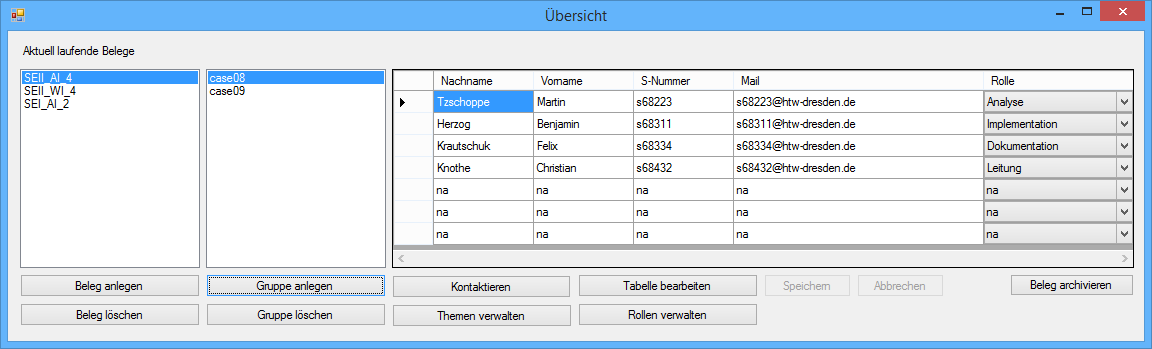
\includegraphics{grafiken/Dozent_Hauptmenue.png}\\
Das Hauptmen� enth�lt zun�chst 2 Listboxen welche die Belege des aktuellen
Semesters anzeigen, sowie die Gruppen des aktuell ausgew�hlten Beleges.
Der Datagridview rechts neben den beiden Listboxen stellt die f�r den Beleg
relevanten Informationen der einzelnen Studenten der aktuell ausgew�hlten
Case-Gruppe dar. Beim Anklicken einer Case-Gruppe wird die Tabelle entsprechend
aktualisiert.\\Im unteren Bereich des Men�s sind einige Buttons zur
Beleg-Verwaltung zu finden.

\subsection{Men�: Beleg anlegen}
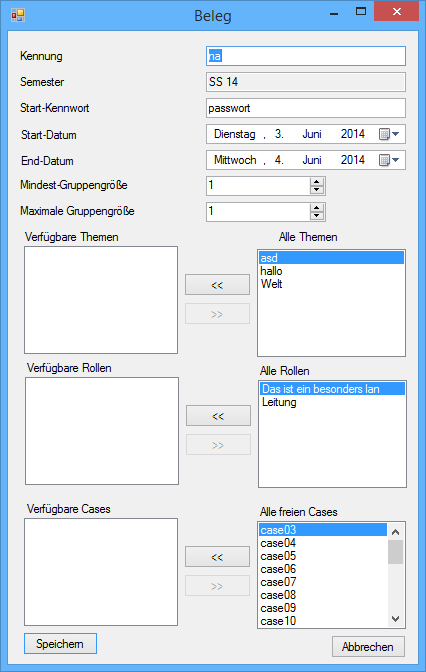
\includegraphics{grafiken/Dozent_Beleg_anlegen.png}\\
Dieses Men� erlaubt es einen neuen Beleg f�r das aktuelle Semester, welches in
der zweiten Zeile angezeigt wird, anzulegen. Der Dozent kann hier das
Startpasswort f�r den Beleg, sowie den Zeitraum und die Gruppengr��e
festlegen.\\Im unteren Bereich dieses Fensters k�nnen speziell f�r diesen Beleg
die w�hlbaren Themen, die festzulegenden Rollen/Verantwortlichkeiten und die
Case-Gruppen ausgew�hlt werden. Der Nutzer kann dabei die gew�nschten Elemente
aus der rechten Seite per Button auf die linke Seite schieben um die speziell
f�r diesen Beleg verf�gbaren Themen, Rollen und Cases festzulegen.
Ein Beleg kann per Doppelklick auf den entsprechenden Beleg in der linken
Listbox bearbeitet werden.


\subsection{Beleg l�schen}
Falls der Beleg noch Case-Gruppen erh�lt wird der Dozent nach Bet�tigen des
L�schen-Buttons eine Warnung. Bei erneuter Best�tigung werden die Belege mit
s�mtlichen Case-Gruppen und gegebenenfalls deren Studenten gel�scht.


\subsection{Gruppe anlegen}
Falls f�r einen Beleg nicht bereits alle Case-Gruppen vergeben sind, kann per
Klick auf den Gruppe-anlegen-Button eine neue Case-Gruppe f�r den Beleg
hinzugef�gt werden.\\
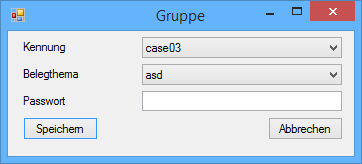
\includegraphics{grafiken/Dozent_Gruppe_anlegen.png}\\
Hier kann die Kennung der anzulegenden Gruppe, das Thema sowie ein Passwort
ausgew�hlt werden.

\section{Programm Student}
.


\end{document}